\documentclass[a4paper,12pt]{article}
\usepackage[utf8x]{inputenc}
\usepackage[T1]{fontenc}
\usepackage[french]{babel}
\usepackage{graphicx}
\graphicspath{ {images/} }
\usepackage{float}
\usepackage{listings}

\setlength{\parindent}{0cm}
\setlength{\parskip}{1ex plus 0.5ex minus 0.2ex}

\title{Organisation de travail}
\author{Mohammad Nauval}

\begin{document}
\maketitle

Dans cette partie, nous allons examiner l'organisation de notre projet. Comme la taille du projet est assez grande et il y a six personnes dans notre équipe, le projet est découpé en plusieurs modules. Les modules sont :

\begin{enumerate}
	\item Analyseur
	\item Compilateur
	\item Interpréteur Minijaja
	\item Interpréteur Jajacode
	\item L'état mémoire
	\item Contrôle de type
	\item Interface homme-machine
\end{enumerate}

Nous avons implémenté l'approche d'agilité dans l'organisation du travail de notre projet. Nous organisons le développement en cycles de quelques semaines. 

Nous avons eu 12 semaines pour finir le projet. Au début du développement, nous avons planifié deux \textit{releases} pour livrer le projet. C'est-à-dire que nous avons eu 6 semaines avant chaque \textit{release}.  

Pour \textit{release} 1, nous avons décidé de réaliser toutes les fonctionnalités du projet. Cependant, celle-ci n'étais logiquement pas possible. En effet, le projet livré pour \textit{relase} 1 n'a pas couvert la totalité de grammaire Minijaja, il fonctionne pour une grammaire réduite. Ensuite, Le projet était élargi pour couvrir la grammaire complète pour \textit{release} 2.

Avant le développement, nous avons défini des fonctionnalités que notre projet doit accomplir. Les fonctionnalités sont ensuite découpées pour chaque \textit{release}. En effet, nous avons les fonctionnalités à accomplir pour \textit{release} 1 ainsi pour \textit{release} 2. Ces fonctionnalités sont définies dans le \textit{backlog} du produit. À partir du backlog produit, nous avons pu définir les \textit{backlog} de \textit{release} 1 et 2.

\begin{figure}[H]
\begin{center}
	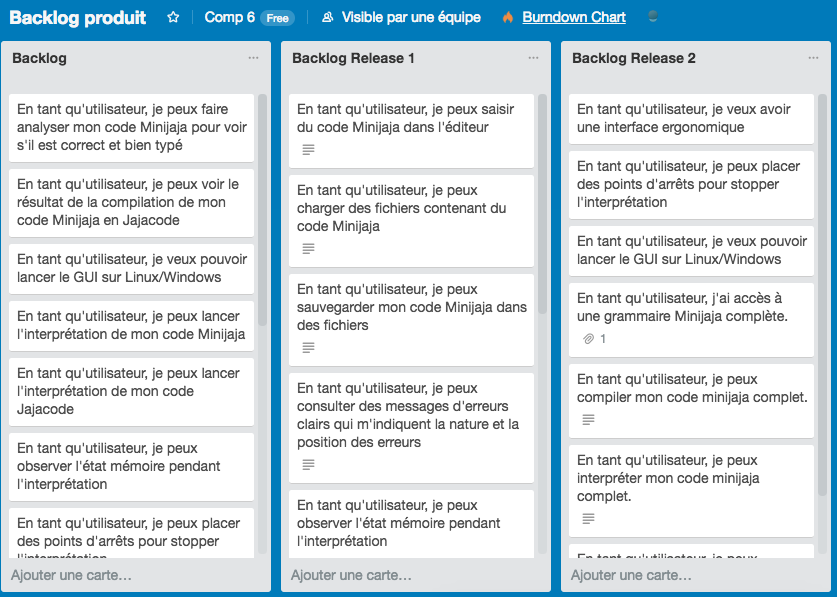
\includegraphics[scale=0.3]{backlogproduit}
	\caption{Backlog produit du projet}
\end{center}
\end{figure}

Comme ce que nous avons déjà mentionné, avec l'approche d'agilité, nous organisons le travail en plusieurs cycles. Les cycles sont appelés des sprints et chaque sprint dure deux semaines. Nous avons donc eu 3 sprint avant chaque \textit{release}. 

Au début de chaque sprint, nous avons organisé une réunion pour définir les tâches que nous avons eu à compléter à la fin du sprint. Pour cela, nous avons examiné le \textit{backlog} de \textit{release} suivant, à partir des fonctionnalités décrites dans ce dernier, nous avons pu extraire les tâches à compléter. Le but c'était de pouvoir implémenter toutes les fonctionnalités décrites dans le backlog de chaque \textit{release} à la fin de trois sprints.

Ensuite, nous avons crée un tableau pour chaque sprint. Dans le tableau, il y a eu trois 4 listes. La première, c'était la liste de tâches à faire. La deuxième et troisième sont la liste de tâches en cours de réalisation et la liste de tâches finies à vérifier. Et la dernière liste, c'était la liste de tâches complétées.

Dans la réunion au début de chaque sprint, chaque membre de l'équipe a choisit les tâches qu'il voulait faire. La réalisation de tâche peut aussi se faire en binôme si sa taille est assez importante. La personne responsable de chaque tâche devait informer son avancement en modifiant l'état de tâche (en cours, à vérifier, ou finie). Pour chaque tâche, nous avons aussi prévu sa durée de réalisation et à la complétion d'une tâche, la durée réelle de ce dernier est aussi révélée.

Par example, voici à ce quoi notre tableau de deuxième sprint de \textit{release} 1 ressemble.

\begin{figure}[H]
\begin{center}
	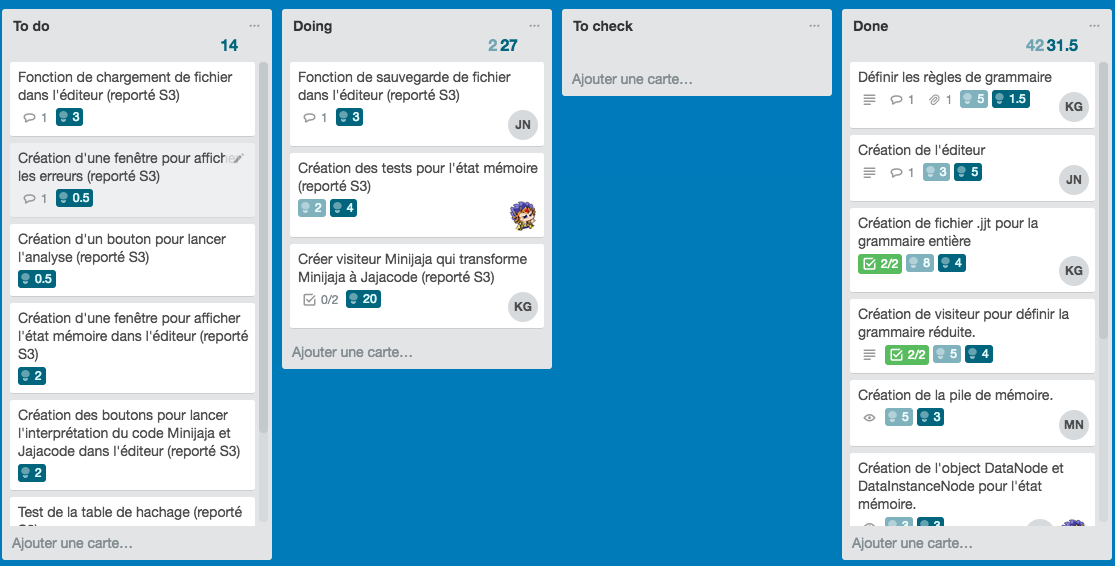
\includegraphics[scale=0.3]{sprint2}
	\caption{Tableau d'organisation de travail de sprint 2 de \textit{release} 1}
\end{center}
\end{figure}

Les tâches non-complétées doivent être reportées au sprint suivant. La personne travaillant sur une tâche doit aussi s'occuper de la réalisation des tests pour vérifier ce qui a été fait.


\end{document}